
\documentclass[12pt]{article} % Use A4 paper with a 12pt font size - different paper sizes will require manual recalculation of page margins and border positions

% Generated with LaTeXDraw 2.0.8
% Mon Jun 17 19:00:40 EDT 2013
\usepackage[usenames,dvipsnames]{pstricks}
\usepackage{epsfig}
\usepackage{pst-grad} % For gradients
\usepackage{pst-plot} % For axes
\usepackage[left=1.3cm,right=4.6cm,top=1.8cm,bottom=4.0cm,marginparwidth=3.4cm]{geometry} % Adjust page margins
\usepackage{amsmath} % Required for equation customization
\usepackage{amssymb} % Required to include mathematical symbols
\usepackage{xcolor} % Required to specify colors by name
\usepackage{amsthm}
\usepackage{float}
\usepackage{tikz}
\usetikzlibrary{shapes,backgrounds,trees}
\usepackage{wasysym}

\makeatletter
\newcommand{\mytag}[2]{%
  \text{#1}%
  \@bsphack
  \protected@write\@auxout{}%
         {\string\newlabel{#2}{{#1}{\thepage}}}%
  \@esphack
}
\makeatother

\setlength{\parindent}{0cm} % Remove paragraph indentation
\newcommand{\tab}{\hspace*{2em}} % Defines a new command for some horizontal space
%\newcommand{\choose}[2]{\left(\begin{matrix}
%{#1}\\{#2}
%\end{matrix}\right)}

\title{Introduction to Probability Theory - Lecture 9}
%----------------------------------------------------------------------------------------

\newtheorem{defn}{Definition}
\newtheorem{example}{Example}
\newtheorem{prop}{Proposition}
\newtheorem{exer}{Exercises}
\newtheorem{thm}{Therorem}
\begin{document}
\maketitle
\section{Common Discrete Distributions - Continued}
Our last common discrete distribution is the \emph{Discrete Uniform} distribution.\\\\
\begin{defn}
Let $C$ be a finite set of numbers and let $X$ be a number chosen from $C$ at random (i.e. each number has equal probability of being selected). Then $X$ has the \emph{Discrete Uniform} distribution, written:
$$X\sim Unif(C)$$
\end{defn}
Clearly, the pmf of $X$ is given by:
$$P(X=x) = \frac1{|C|}$$
\begin{example}
Let $C =\left\{1,2,...,10\right\}$ Then
$$P(X=4) = \frac1{10}$$
\end{example}
\section{Cumulative Distribution Function - CDF}
\begin{defn}
The CDF of a random variable $X$ is the function:
$$F(x) = P(X\leq x)$$
\end{defn}
\begin{example}
Let $X\sim Bin(n,p)$.
$$F(3) = P(X\leq 3) = P(X=0)+P(X=1)+P(X=2)+P(X=3) = \sum_{k=0}^3{n\choose{k}}p^kq^{n-k}$$
In general, the Binomial CDF is given by:
$$F(x) = \sum_{k=0}^x {n\choose{k}}p^kq^{n-k}$$
\end{example}
CDFs are most useful in the context of \emph{continuous} random variables, so we will state its defining properties here, but we will discuss it further in the continuous context.
\begin{thm}
Any CDF, $F$, has the following properties:
\begin{enumerate}
\item $F$ is increasing, i.e. if $x_1<x_2$ then $F(x_1)\leq F(x_2)$
\item $F$ is right-continuous, i.e.
$$F(a) = \lim_{x\rightarrow a^+} F(x)$$
\item 
$$\lim_{x\rightarrow -\infty} F(x) = 0$$
and
$$\lim_{x\rightarrow\infty} F(x) = 1$$
\end{enumerate}
\end{thm}
\section{Functions of Random Variables}
There are many contexts in which we will encounter functions of random variables. For example, we will see them when we define conditional expectation and when we study transformations. It is important to note that functions of random variables \emph{are} random variables!
\begin{thm}
Any function $g:\mathbb{R}\rightarrow\mathbb{R}$ of a random variable is a random variable.
\end{thm}
\begin{proof}
A random variable $X$ is a function that takes events in $\mathcal{E}$ and returns a real number. A function $g$ applied to a random variable $X$ is the composition: 
$$g\circ X:\mathcal{E}\rightarrow \mathbb{R}$$
\end{proof}
Now, the transformed random variable does \emph{not} have the same distribution of the original variable, and finding the distribution of the transformed variable can be challenging. We will discuss methods for doing this later when we focus on transformations of random variables. For now, look at the discussion of category errors and sympathetic magic in the text (pg 115).\\\\
We have one final topic to touch on in Chapter 3, and then we talk about expectation and variance.
\section{Independence of Random Variables}
Recall that for events, we defined to events $A$ and $B$ to be independent $iff$
$$P(A\cap B) = P(A)\cdot P(B)$$
We can define a similar concept for random variables. We will define what it means for two \emph{discrete} random variables to be independent now, and we will re-visit this topic after we have studied continuous random variables.\\\\
\begin{defn}
Two discrete random variables $X$ and $Y$ are independent if for all possible values $x_1$ of $X_1$, $x_2$ if $X_2$,...,$x_n$ of $X_n$, we have
$$P(X_1=x_1, X_2=x_2, ...,X_n=x_n) = P(X_1=x_1)P(X_2=x_2)...P(X_n=x_n)$$
\end{defn}
Note the following:
\begin{itemize}
\item The commas on the left hand side should be read as 'and'.
\item The $x_i$'s stand for all possible values that the corresponding random variable $X_i$ can take. Thus, if the support of $X_1$ is say $0,1,2,3$, then the above equality would have to hold for $X_1=0,X_1=1,X_1=2,X_1=3$.
\item  This is slightly different than our definition for the independence of multiple events - there we required the probability of any possible intersections of events must factor into a product of their individual probabilities. Here, we specify what \emph{looks likes} only one combination. However, because this needs to hold for all possible combinations of possible values of the $X_i$, we really have the same kind of requirement.
\item Pairwise independence \emph{does not} imply independence.
\item Independence \emph{does} imply pairwise independence.
\end{itemize}
This completes our coverage of chapter 3 in the text. 
\section{Expectation and Variance}
Expectation and variance are the first of several 'summary' properties of distributions we will study. We will be interested in such properties as the center, the spread, symmetry vs. skewness, etc., in addition to parameters that shift or scale distributions.\\\\
\begin{defn}
Let $X$ be a discrete random variable with pmf $f(x)$. The \emph{expected value} of $X$ is defined to be:
$$E(X) = \sum_x x f(x)$$
where the sum is over all possible values of $X$.
\end{defn}
\begin{example}
Toss a (fair) coin two times. Let $X$ be the number of heads. We know that $X\sim Bin(2,\frac12)$. Thus, the pmf of $X$ is
$$f(x;p) = {n\choose{x}}p^xq^{n-x} = {2\choose{x}}\left(\frac12\right)^2$$
and
$$E(X) = \sum_{x=0}^2 x {2\choose{x}}\left(\frac12\right)^2 = 0 + {2\choose{1}}\left(\frac12\right)^2 + 2{2\choose{2}}\left(\frac12\right)^2= \frac12 + \frac12 = 1$$
\end{example}
In general, we can compute the expectation of a Binomial random variable in terms of its parameters $n$ and $p$. I.e., let $X\sim Bin(n,p)$:
\begin{eqnarray*}
E(X) &=& \sum_{x=0}^n x {n\choose{x}}p^xq^{n-x}\\
&=& \sum_{x=1}^n x {n\choose{x}}p^xq^{n-x} \textrm{ the zeroth term is zero}\\
&=& \sum_{x=1}^n {n\choose{x-1}}p^xq^{n-x} \textrm{ bring the }x\textrm{ term inside the combination}\\
&=& \sum_{x=1}^n \frac{n!}{(n-(x-1))!(x-1)!}p^xq^{n-x} \textrm{ just expand the combination}\\
&=&np \sum_{x=1}^n \frac{(n-1)!}{(n-(x-1))!(x-1)!}p^{x-1}q^{n-x} \textrm{ factor out an }n \textrm{ and a } p\\
&=&np \sum_{k=0}^n \frac{(n-1)!}{(n-k)!k!}p^kq^{n-(k+1)} \textrm{ set }k=x-1\textrm{ and re-index the sum}\\
&=&np \sum_{k=0}^n \frac{(n-1)!}{(n-k)!k!}p^kq^{n-1+k}\\
&=& np
\end{eqnarray*}
where the last term follows because 
$$\sum_{k=0}^n \frac{(n-1)!}{(n-k)!k!}p^kq^{n-1+k} = (p+q)^{n-1} = 1$$
\subsection{Properties of Expectation}
Expectation has several important properties that we will be using \emph{a lot}!
\begin{itemize}
\item $E(X)$ is \emph{linear}. This means that for any two random variables $X$ and $Y$ and any scalar (i.e. number) $a$ we have:
$$E(X+Y) = E(X) + E(Y)$$
and
$$E(aX) = aE(X)$$.
These follow directly from the definition of expectation (sums are linear).
\item $E(X)$ can be thought of as a \emph{weighted average}. Note that when we average a set of numbers, we add them together and divide by how many numbers there are. This can be interpreted as an expectation, where all numbers have equal probability. In other words, we are summing the numbers, weighted by their probability, which is $1/n$ for a set of $n$ numbers. In fact, the usual 'average' or 'mean' of a set of numbers is the expectation of a random variable with a discrete uniform distribution on that set of numbers. 
\item $E(X)$ is a measure of the \emph{center} of a distribution, or the center of mass (where probability is thought of as mass). For example, consider the following histograms:
\begin{minipage}{3in}
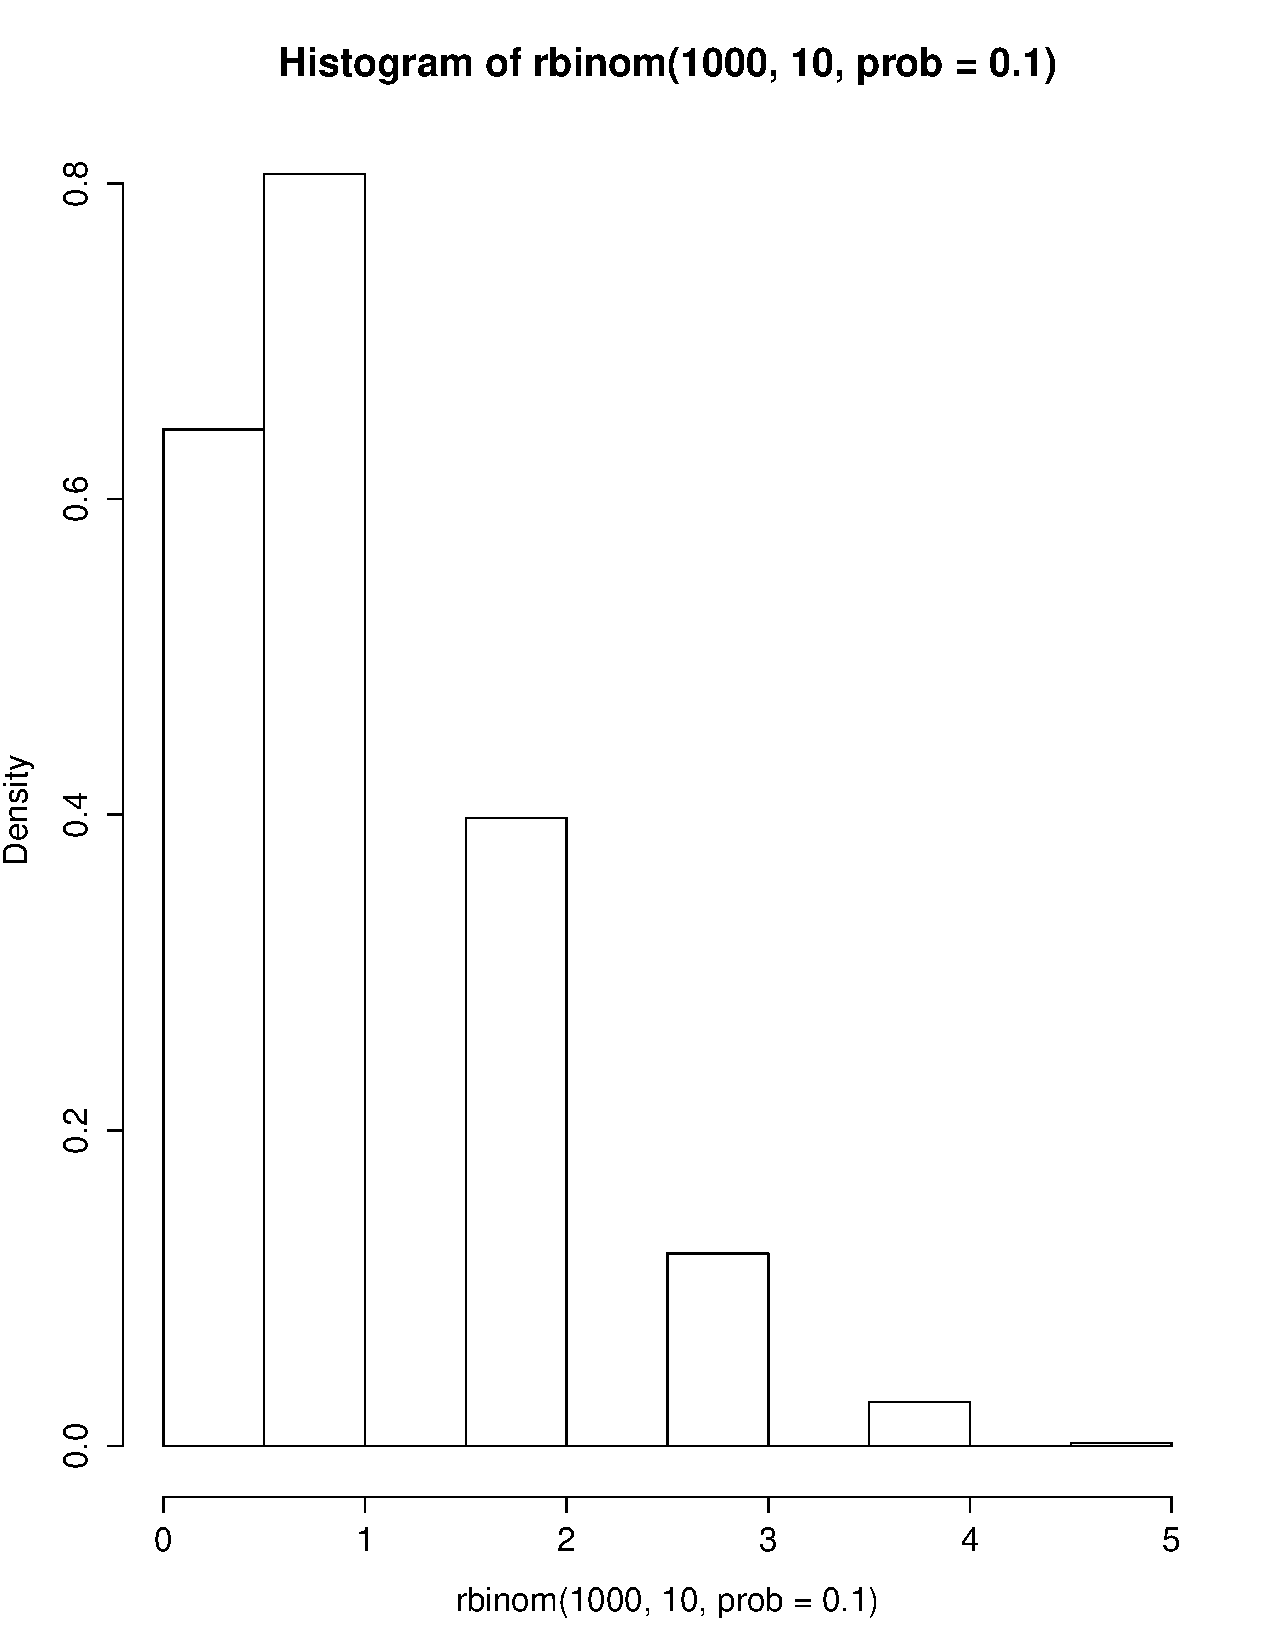
\includegraphics[width=2.9in]{rbinom.pdf}
\end{minipage}
\begin{minipage}{3in}
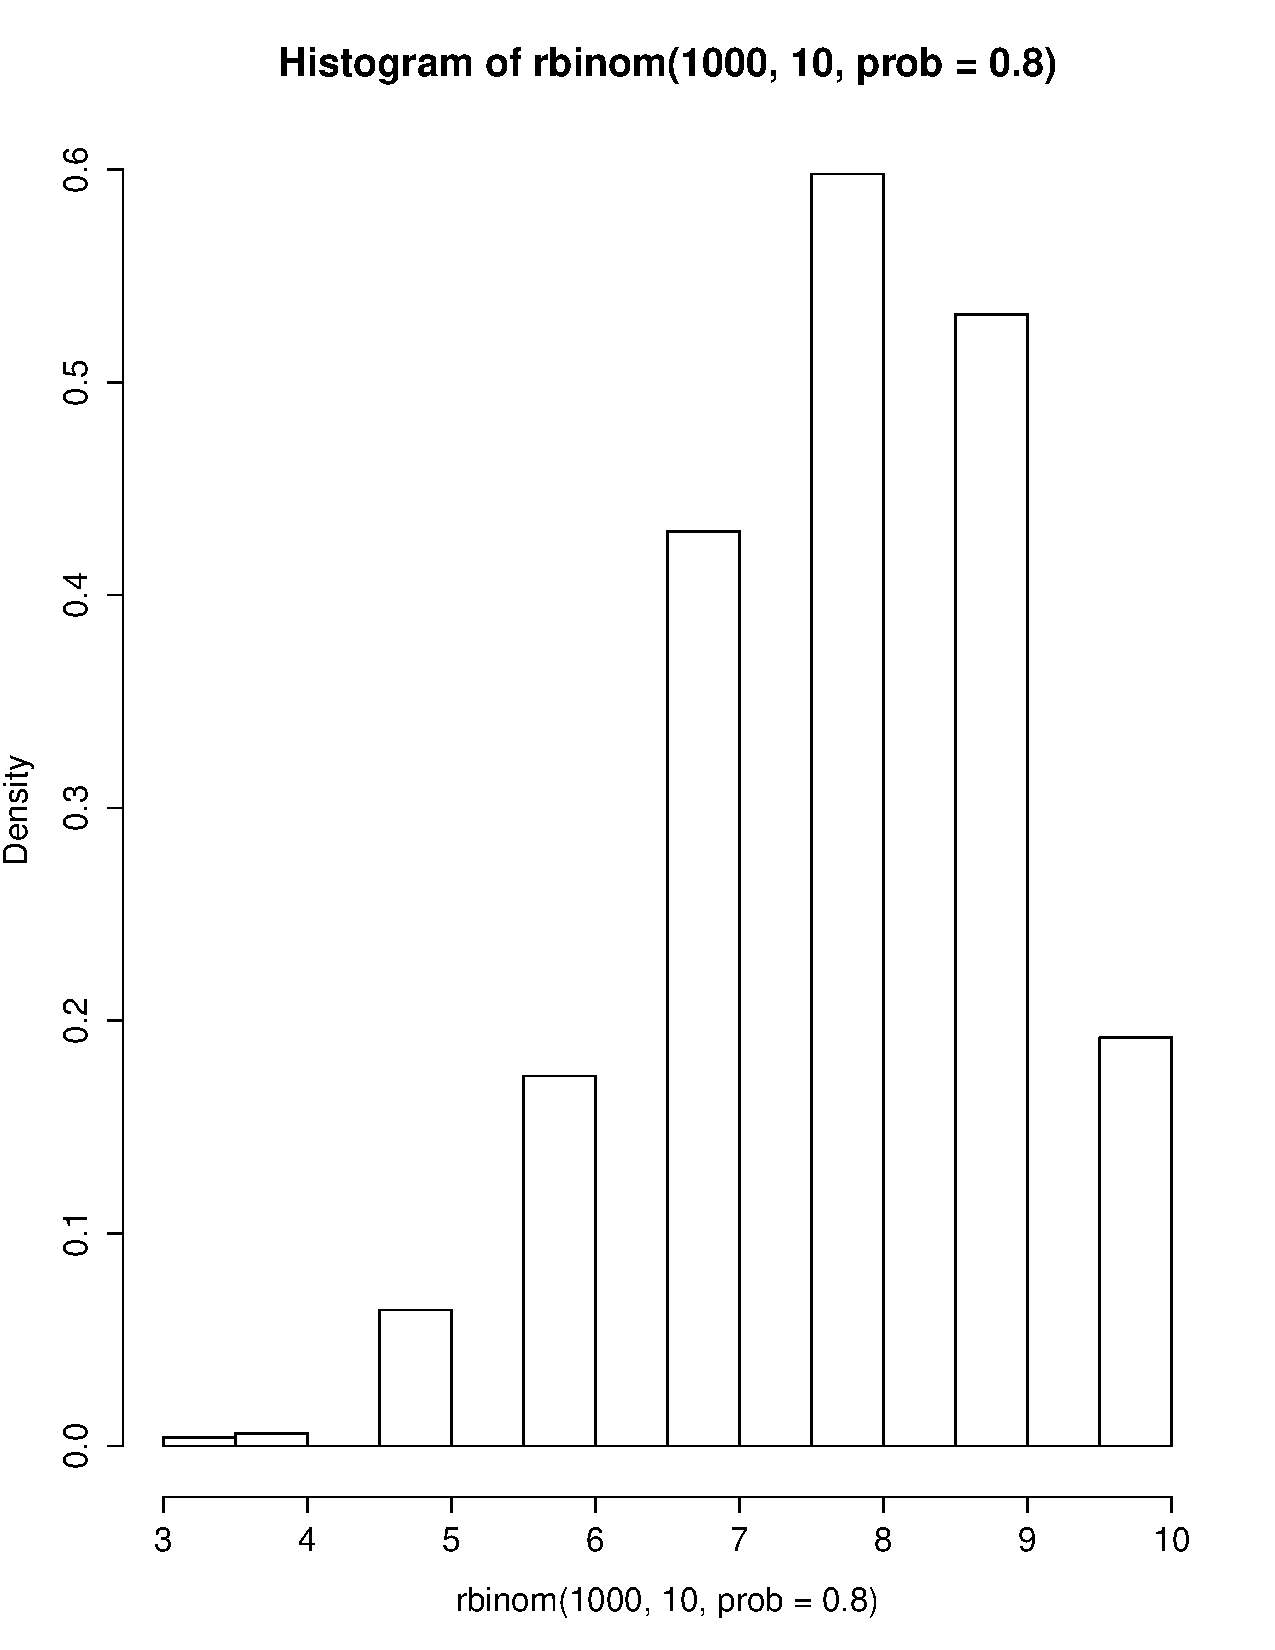
\includegraphics[width=2.9in]{rbinom_8.pdf}
\end{minipage}
We have just shown that the expected value of a Binomial random variable is $np$. In the histogram on the left, the expected value is $1$. Notice how the frequency is 'centered' near $X=1$. Similarly, in the histogram on the right, the expected value is $8$, and the frequency is centered near $X=8$.
\item  $E(X)$ need not be a possible value of $X$. Consider a die roll and let $X=$ number rolled. There are $6$ outcomes, all equally likely (probability $\frac16$), thus
$$E(X) = \frac16\left(1+2+3+4+5+6\right) = 3.5$$
\item $E(X)$ depends only upon the \emph{distribution} of $X$. Recall that two different random variables $X$ and $Y$ can have the same distribution. If $X$ and $Y$ have the same distribution, then $E(X) = E(Y)$.
\item For any function $g:\mathbb{R}\rightarrow \mathbb{R}$ and any random variable $X$ with pmf given by $f(x)$, we have:
$$E(g(X)) = \sum_x g(x) f(x)$$
\end{itemize}
\end{document}